\chapter{Einleitung}
\label{chapter:Einleitung}

\section{Motivation der Hyperloop Technologie}
\label{section:Motivation}

Der Hyperloop ist ein innovatives Transportkonzept, dass eine ökonomische, klimafreundliche und schnellere Alternative zu herkömmlichen Verkehrsmitteln wie Lastkraftwagen, Zügen und Flugzeugen bietet.\\
\pagebreak[3]
\begin{figure}[!ht]
	\begin{center}
		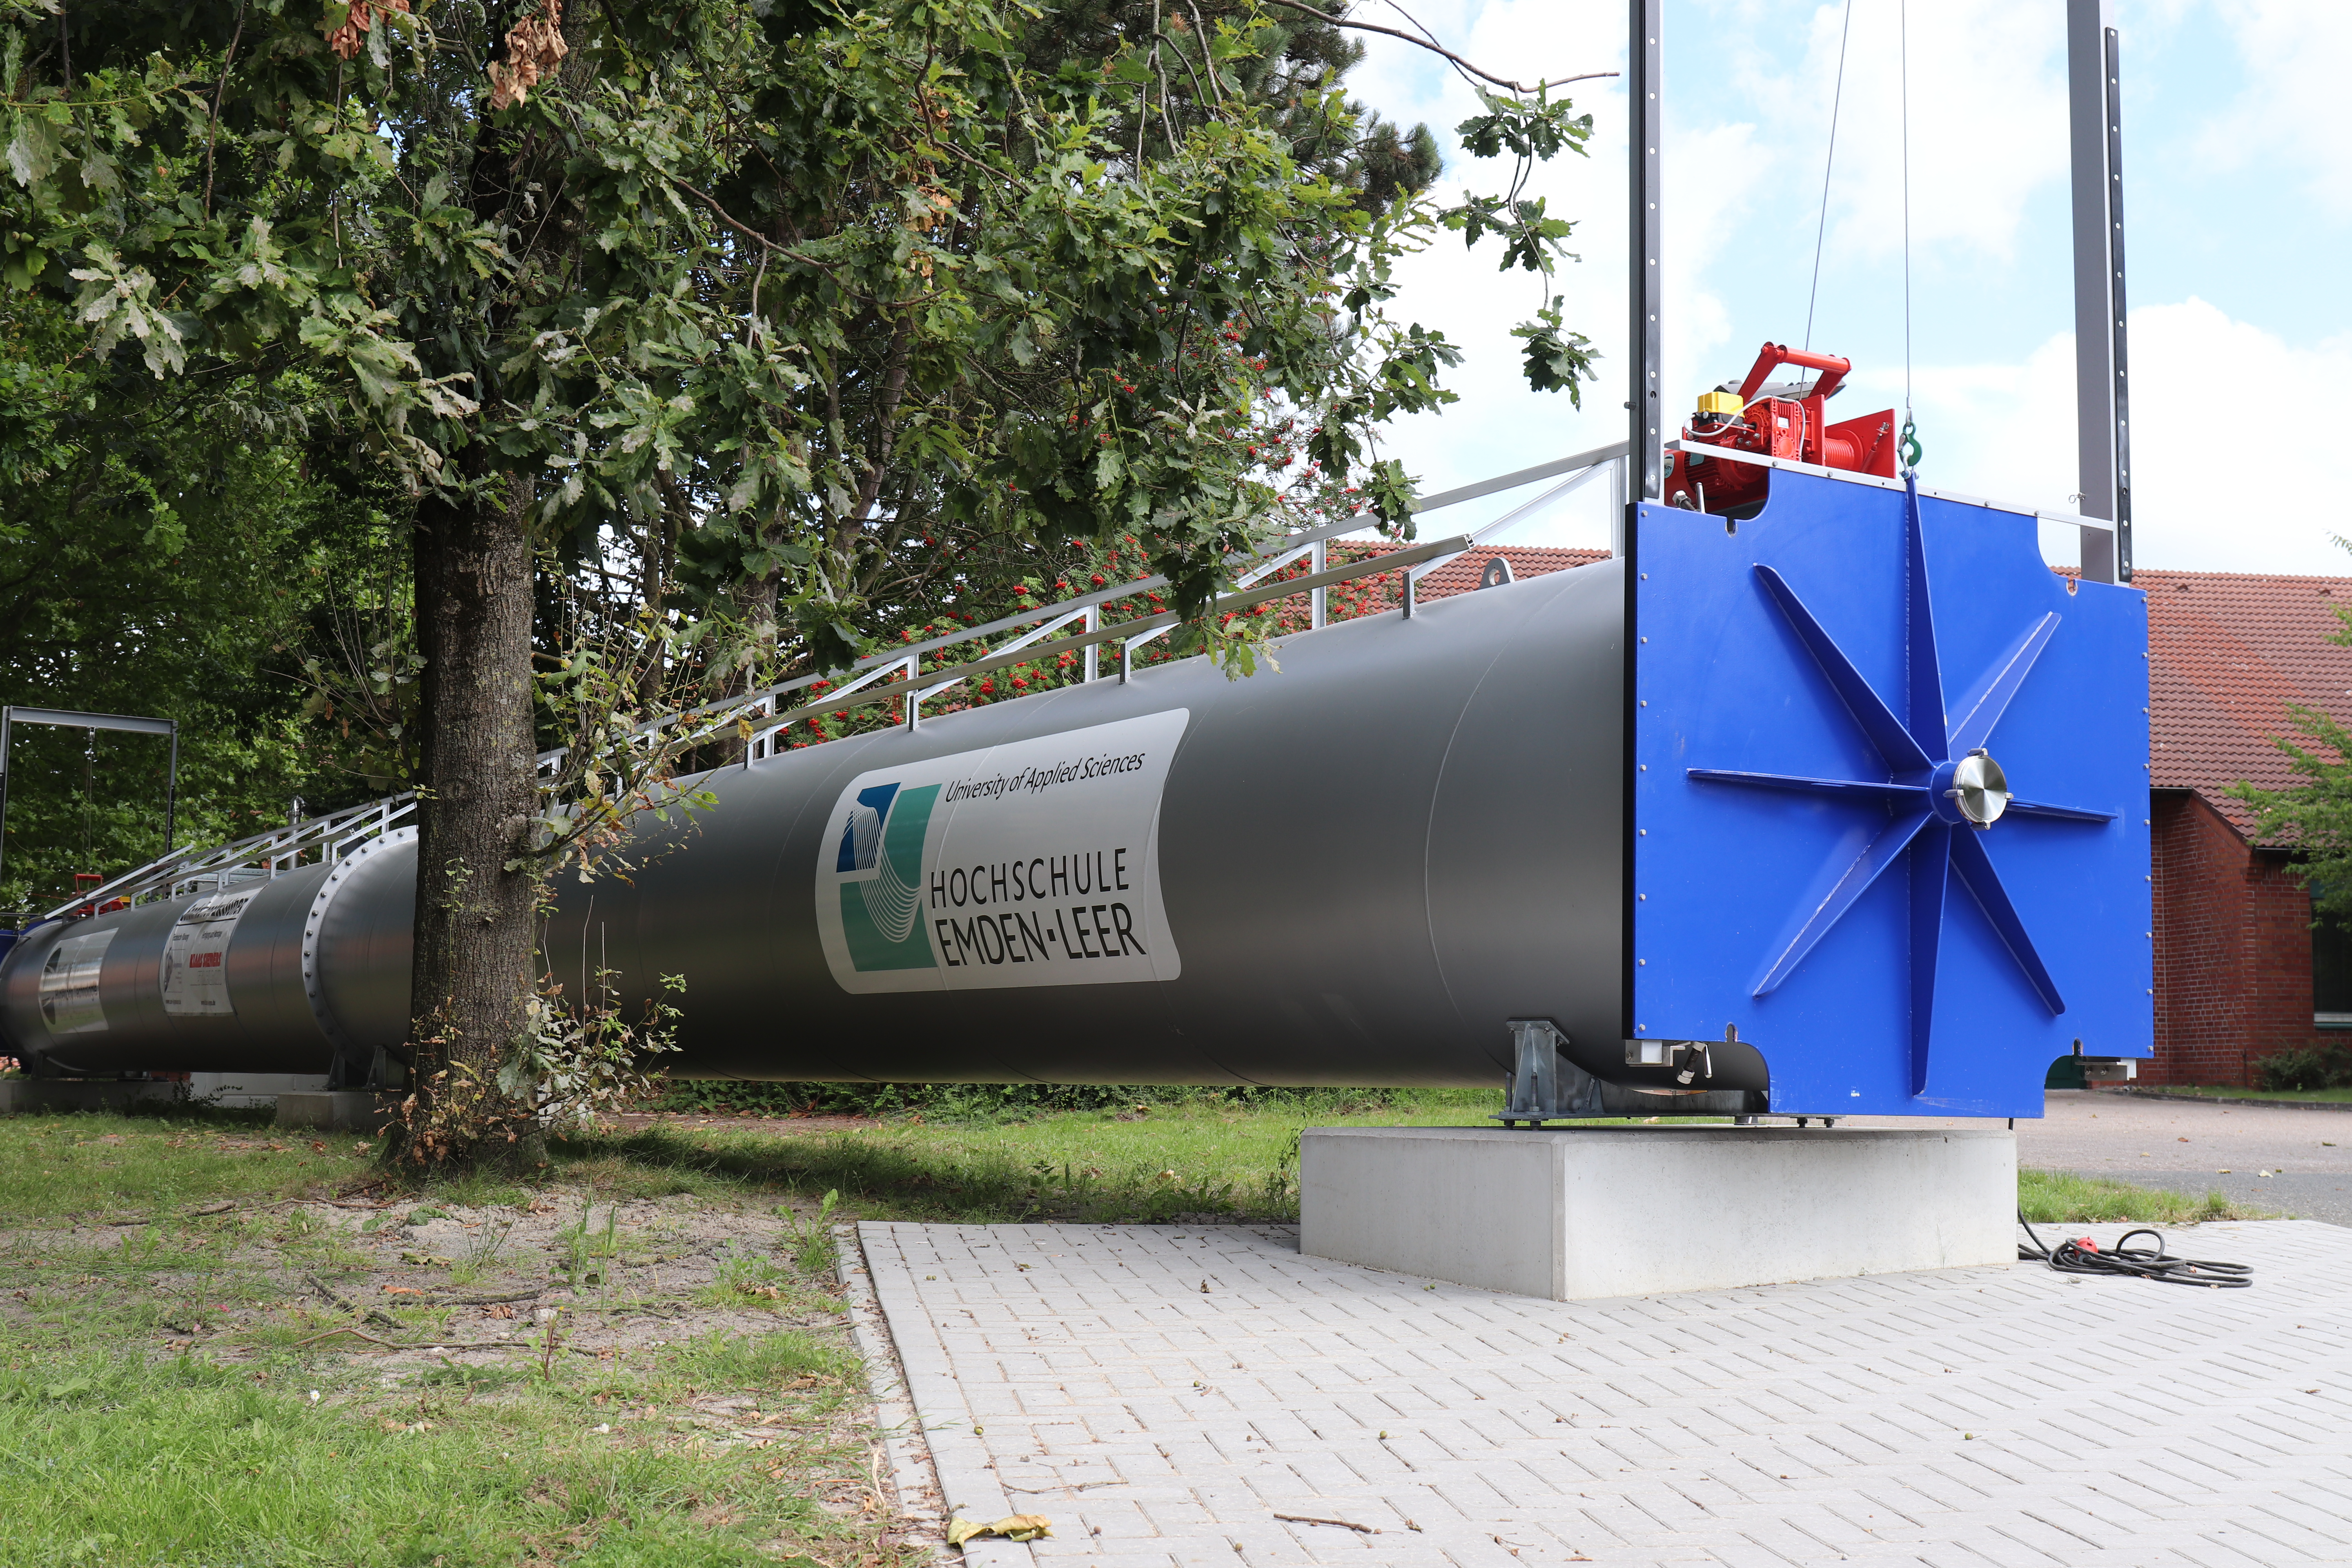
\includegraphics[width=1\textwidth]{img/1_strecke/strecke_1.png}
		\caption{Hyperloop der Hochschule Emden-Leer}
		\label{img_1_1:strecke}
	\end{center}
\end{figure}
\pagebreak[4]
Derzeit stehen herkömmlichen Transportmitteln zwei wesentliche Hindernisse im Weg, um Personen oder Güter schnell und emissionsarm zu befördern: Zum einen der hohe Luftwiderstand, der bei hohen Geschwindigkeiten den Energieverbrauch stark erhöht, und zum anderen der Rollwiderstand der Räder, der ebenfalls zu einem höheren Energiebedarf führt.\\


Der Hyperloop löst diese Probleme, indem er Güter und Personen in einem Fahrzeug, das sich in einer Vakuumröhre bewegt, wie in Abbildung \ref{img_1_1:strecke} dargestellt ist. Zudem wird das Fahrzeug, wie bei einer Magnetschwebebahntechnik angehoben. Somit lassen sich Roll- und Luftwiderstand fast vollkommen aufheben.



%%%%%%%%%%%%%%%%%%%%%%%%%%%%%%%%%%%%%%%%%%%%%%%%%%%%%%%%%%%%%%%%%%%%%%%%%%%%%%%%%%%%
%%%%%%%%%%%%%%%%%%%%%%%%%%%%%%%%%%%%%%%%%%%%%%%%%%%%%%%%%%%%%%%%%%%%%%%%%%%%%%%%%%%%
%%%%%%%%%%%%%%%%%%%%%%%%%%%%%%%%%%%%%%%%%%%%%%%%%%%%%%%%%%%%%%%%%%%%%%%%%%%%%%%%%%%%
%%%%%%%%%%%%%%%%%%%%%%%%%%%%%%%%%%%%%%%%%%%%%%%%%%%%%%%%%%%%%%%%%%%%%%%%%%%%%%%%%%%%
%%%%%%%%%%%%%%%%%%%%%%%%%%%%%%%%%%%%%%%%%%%%%%%%%%%%%%%%%%%%%%%%%%%%%%%%%%%%%%%%%%%%
%%%%%%%%%%%%%%%%%%%%%%%%%%%%%%%%%%%%%%%%%%%%%%%%%%%%%%%%%%%%%%%%%%%%%%%%%%%%%%%%%%%%



\subsection{Institute of Hyperloop Technology}
\label{section:IHT}

%Die Hochschule Emden/Leer hat im Jahr 2021 das Institut für Hyperloop-Technologie (IHT) gegründet, um aktiv an der Forschung zu dieser zukunftsweisenden Technologie teilzunehmen.

Im Rahmen dieser Forschung wurde an der Hochschule Emden eine Teststrecke mit einer Länge von 27 Metern errichtet (siehe Abbildung \ref{img_1_1:strecke}). Auf dieser Strecke soll das Fahrzeug (Pod) unter realistischen Bedingungen getestet und weiterentwickelt werden.
Die Teststrecke besteht aus einem Schienensystem und einem Linearmotor.

\newpage




\section{Aufgabenstellung}
\label{section:Aufgabenstellung}

\myboxy{
	\begin{itemize}
		\item Ablauforientiert erklären. Also erst die Bestellung, dann der Schaltplan und dann die Simulation mit Simulink.
		\item Aufgabenstellung in der Vergangenheit formulieren.
		\item Den Leser in der Doku struktur Einführen. Am enden in 1.x
	\end{itemize}
}{To-do}{\textwidth}


Die Motivation für dieses Projekt liegt in der Entwicklung eines Hyperloop-Fahrzeugs, das mit einer Batterie und einem Motor betrieben wird. Für die Steuerung des Fahrzeugs wurde ein echtzeitfähiges Steuerungsystem der Firma Speedgoat vorgeben, welches in Abschnitt \ref{section:speedgoat} vertieft wird.\\ \ \\

Im Rahmen des Projekts wird ein Fahrzeug (Pod) für den Hyperloop mit einer Bordspannung von 48 V konzipiert. Ziel ist es, die Realisierbarkeit dieser Spannung zu überprüfen und umzusetzen. Dazu gehören die Planung und Simulierung, die Integration der erforderlichen Sensorik sowie die Beschaffung der notwendigen Bauteile. Die Logik- und Signalverarbeitung wird mithilfe von Simulink auf dem echtzeitfähigen Speedgoat-System durchgeführt.
Die Steuerung erfolgt über Simulink, ein Modul von MATLAB, und umfasst die Erfassung von Position und Beschleunigung des Fahrzeuges. Der Motor wird über ein zusätzliches Steuergerät angesteuert. Die Steuerung soll in Form einer Automatensteuerung umgesetzt werden.
Die Verdrahtung des Pods wird entsprechend der Bordspannung von 48 V ausgelegt. Hierfür wird mit der Software QElectroTech ein Schaltplan (siehe Anhang \ref{Anhang:Schaltplan}) erstellt.
Alle erforderlichen Bauteile für die Umsetzung der Bordspannung, die Verdrahtung und die Sensorik müssen beschafft werden.\\
Textergebnisse und Inbetriebnahme entfallen.


%%%%%%%%%%%%%%%%%%%%%%%%%%%%%%%%%%%%%%%%%%%%%%%%%%%%%%%%%%%%%%%%%%%%%%%%%%%%%%%%%%%%
%%%%%%%%%%%%%%%%%%%%%%%%%%%%%%%%%%%%%%%%%%%%%%%%%%%%%%%%%%%%%%%%%%%%%%%%%%%%%%%%%%%%
%%%%%%%%%%%%%%%%%%%%%%%%%%%%%%%%%%%%%%%%%%%%%%%%%%%%%%%%%%%%%%%%%%%%%%%%%%%%%%%%%%%%
%%%%%%%%%%%%%%%%%%%%%%%%%%%%%%%%%%%%%%%%%%%%%%%%%%%%%%%%%%%%%%%%%%%%%%%%%%%%%%%%%%%%
%%%%%%%%%%%%%%%%%%%%%%%%%%%%%%%%%%%%%%%%%%%%%%%%%%%%%%%%%%%%%%%%%%%%%%%%%%%%%%%%%%%%
%%%%%%%%%%%%%%%%%%%%%%%%%%%%%%%%%%%%%%%%%%%%%%%%%%%%%%%%%%%%%%%%%%%%%%%%%%%%%%%%%%%%

\section{Aufbau der Projektdokumentation}
\label{section:Aufbau}

\myboxy{
	\begin{itemize}
		\item Wird am Ende geschrieben.
	\end{itemize}
}{To-do}{\textwidth}



%%%%%%%%%%%%%%%%%%%%%%%%%%%%%%%%%%%%%%%%%%%%%%%%%%%%%%%%%%%%%%%%%%%%%%%%%%%%%%%%%%%%
%%%%%%%%%%%%%%%%%%%%%%%%%%%%%%%%%%%%%%%%%%%%%%%%%%%%%%%%%%%%%%%%%%%%%%%%%%%%%%%%%%%%
%%%%%%%%%%%%%%%%%%%%%%%%%%%%%%%%%%%%%%%%%%%%%%%%%%%%%%%%%%%%%%%%%%%%%%%%%%%%%%%%%%%%
%%%%%%%%%%%%%%%%%%%%%%%%%%%%%%%%%%%%%%%%%%%%%%%%%%%%%%%%%%%%%%%%%%%%%%%%%%%%%%%%%%%%
%%%%%%%%%%%%%%%%%%%%%%%%%%%%%%%%%%%%%%%%%%%%%%%%%%%%%%%%%%%%%%%%%%%%%%%%%%%%%%%%%%%%
%%%%%%%%%%%%%%%%%%%%%%%%%%%%%%%%%%%%%%%%%%%%%%%%%%%%%%%%%%%%%%%%%%%%%%%%%%%%%%%%%%%%